\chapter{不相交路径问题}


不相交路径(Disjoint Path) 问题可以看作是最短路径问题的一个扩展。是计算出几条不共享任何公共点/边的路径。提供不相交路径将提高网络连接的可靠性和网络流量,并相应地提高网络的可生存性。网络可生存性被定义为在网络组件(例如,节点/链路)发生故障时提供持续服务的能力\cite{zhou2000survivability}。 不相交路径对问题是不相交路径问题的另一个变体。

不相交路径具有广泛的应用域。例如,对于通信网络中的业务具有多条不相交的路径将提高其传输可靠性。通过在多个不相交路径上并发发送流量,路径的失败不会影响其他路径的性能,并且流量仍将到达其目的地。在交通网络中,预先计算出的不相交路径数将使卡车司机能够按照不同的路径改变路线,而不是总是坚持最短的路径。

%maritime network freights

本章的其余部分按以下方式组织。在\textbf{不相交路径}部分,给出了不相交路径的形式化定义,讨论不相交路径问题的附加条件限制及其相应的复杂性,描述几种有代表性的不相交路径算法。在\textbf{基于可靠性的不相交路径}部分,我们将介绍路径可靠性的概念及其与不相交路径的关系。在\textbf{最大不相交路径}部分将阐述不相交路径可能部分重叠的情况下而不是完全不相交。在域不相交路径章节,我们继续寻找域不相交路径在多域网络中。因为多个链接(或多个节点)可能在共享风险下同时失败,在\textbf{共享风险链接组不相交路径}部分介绍共享风险链接组SRLG 的概念。确保不相交的路径不会同时失效由于单个链接(或节点)失败。风险也可能影响基于地区的网络,因此\textbf{地区不相交路径}部分讨论了几种基于地区的风险模型。与不相交路径问题对应的不相交路径对问题将在\textbf{不相交路径对}部分中讨论,将讨论不同情况下的复杂性。最后,我们在最后一节对本章进行了简要的总结。

\section{预备知识}
%\subsection{图论}
网络在我们的日常生活中非常普遍。我们的身体组成突触连接的神经元网络。我们的运输网络使我们能够轻松地往返于不同的地方。互联网是我们巨大的信息门户也是世界域内的计算机网络。电网提供电力,而如果没有电力那我们现在社会都可能会停止运作。我们的社交网络让我们和朋友与家人联系。由于网络的重要性,网络特性的多样性已经得到了广泛的研究,尤其是在图论领域。

在图论中,网络被看作是一种通过节点互相链接的。节点表示网络的关节点,例如,通信网络中的路由器,海运网络或交通网络中的城市。链路表示将关键点连接在一起的连接器,例如,通信网络中的电缆,海运中的贸易路线,运输网络中的网络或公路。

图论中研究最多的课题之一是最短路径问题,即在网络中的两个节点,使得路径上链路权重之和最小化。传统的最短路径算法是Dijkstra算法\cite{dijkstra1959note}以及Bellman-Ford 算法\cite{toth2002vehicle,ford2015flows}。 使用最短路径,在一个通信网络的两个路由器间信号可以在最小延迟之间交换,货物可以在海运网络中两个港口之间的以燃油成本最低的代价发送,而且在运输网络中我们可以更快地往返于城市之间。

网络通常表示为图$G(\mathbb{V},\mathbb{E})$,其中$\mathbb{V}$是$|\mathbb{V}|$ 个节点的集合(例如,节点表示路由)和$\mathbb{E}$是$|\mathbb{E}|$ 条链路的集合(例如,链路代表光纤线路或无线电信道)。链接可能带有延迟、长度或成本等属性。对于每条链路$e_i$,$w_{e_i}$表示链路的权重。路径$P$的权重表示为路径$P$中每条链路的权重之和$w_P=\sum\limits_{e_i\in \mathbb{P}}w_{e_i}$。
\section{不相交路径}
不相交路径问题被定义成如下:

\begin{definition}[不相交路径问题]
给定$|\mathbb{V}|$个节点集$\mathbb{V}$和 $|\mathbb{E}|$条加权链集 $\mathbb{E}$ 组成的有向网络 $G(\mathbb{V},\mathbb{E})$,两个特殊节点$s,d\in\mathbb{V}$。 给定一个整数$k>0$,求$s$到$d$的$k$ 条路径$P_1,P_2,\ldots,P_k$,使路径间不共享任何公共链接(或节点)。
\end{definition}

对不相交的路径施加附属目标条件,例如:
\begin{itemize}
  \item 最小-最大不相交路径问题--最大路径的所有链路权重之和最小化。
  \item 最小-最小不相交路径问题--最小路径的所有链路权重之和最小化。
  \item 有界不相交路径问题--每条路径的所有链路权重之和应小于给定权值$\bigtriangleup$.
  \item 最小和不相交路径问题--k条路径的所有链路权重之和的总和最小化。
\end{itemize}
在算法1中示出了求解不相交路径问题的简单启发式算法,我们将称之为迭代DP 算法。
迭代DP算法基于K个连续最短路径计算的使用

\begin{algorithm}[!h]
{
{
\renewcommand\baselinestretch{1.5}\selectfont %控制行距
\caption{ Scheduling Algorithm }
\label{alg:schedule}
\begin{algorithmic}[1]
\REQUIRE ~\\
A DFG $G=<V,E>$;\\
An allocation $A(G)$ for $G$.
\ENSURE ~\\
A schedule.
    \STATE{.......................}
    \FOR{$i\leftarrow\ 1\ to\ M$}
        \STATE{.......................}
    \ENDFOR
    \STATE{.......................}
    \STATE{.......................}
    \STATE{.......................}
    \STATE{.......................}
    \STATE{.......................}
    \FOR{$k\leftarrow\ 1\ to\ |V|$}
        \STATE{.......................}
        \STATE{.......................}
        \STATE{.......................}
        \STATE{.......................}
    \IF{$LT_k==j$}
        \IF{there is no idle core in cluster $cl_{loc}$}
            \STATE{.......................}
            \STATE{.......................}
            \STATE{.......................}
            \STATE{.......................}
            \STATE{.......................}
            \STATE{.......................}
        \ELSE
            \STATE{.......................}
            \STATE{.......................}
            \STATE{.......................}
            \STATE{.......................}
            \STATE{.......................}
            \STATE{.......................}
        \ENDIF
    \ENDIF
    \ENDFOR


\end{algorithmic}
}
\par}
\end{algorithm}
\section{可用性不相交路径}
路径可用度是指路径在未来随机时间内处于运行状态的概率\cite{clouqueur2002availability}。 路径$P$的可用度($A$) 可以通过乘以其所有组成链路的可用度来计算:
\begin{equation}
A=\prod_{y\in P}a_yp
\end{equation}

其中$a_y$是链路y的可用度,它依赖于链路的平均故障间隔时间(MTBF)和平均修复时间(MTTR)。
\begin{equation}
a=\frac{MTBF}{MTBF+MTTR}
\end{equation}
\begin{equation}
MTBF=\frac{total\ operating\ time}{number\ of\ failures}=\frac{1}{failure\ rate}
\end{equation}
\begin{equation}
MTTR=failure localization\ time+failure\ repair\ time
\end{equation}
k条不相交路径的总可用度可以计算为:
\begin{equation}
A_t=1-\prod_k(a-A_k)
\end{equation}
可靠性不相交路径问题被定义成如下:

\begin{definition}[可用性不相交路径]
给定$|\mathbb{V}|$个节点集$\mathbb{V}$和 $|\mathbb{E}|$条加权链集 $\mathbb{E}$ 组成的有向网络 $G(\mathbb{V},\mathbb{E})$,两个特殊节点$s,d\in\mathbb{V}$;给定一个整数$k>0$ 和小数$\delta$,每条链路的权重即每条链路的可用度,求$s$ 到$d$ 的$k$ 条路径$P_1,P_2,\ldots,P_k$,使路径间不共享任何公共链接(或节点)并且$k$ 条路径总的可用度$A_t$ 至少为$\delta$。


\end{definition}
\section{最大不相交路径}
最大不相交路径问题被定义成如下:

\begin{definition}[最大不相交路径问题]
给定$|\mathbb{V}|$个节点集$\mathbb{V}$和 $|\mathbb{E}|$条加权链集 $\mathbb{E}$ 组成的有向网络 $G(\mathbb{V},\mathbb{E})$,两个特殊节点$s,d\in\mathbb{V}$;给定一个整数$k>0$,求$s$到$d$的$k$ 条路径$P_1,P_2,\ldots,P_k$,使路径间共享最少的公共链接(或节点)。
\end{definition}
\section{域不相交路径}
域不相交路径问题被定义成如下:

\begin{definition}[域不相交路径问题]
给定$|\mathbb{V}|$个节点集$\mathbb{V}$,$|\mathbb{E}|$条加权链集 $\mathbb{E}$,$|\mathbb{D}p|$个域集$\mathbb{D}$,$|\mathbb{L}|$条域内加权链集 $\mathbb{L}$ 组成的有向网络 $G(\mathbb{V},\mathbb{E},\mathbb{D},\mathbb{L})$,两个特殊节点$s,d\in\mathbb{V}$。每个域$d\in\mathbb{D}$由一组点集$\mathbb{V}_d\subseteq \mathbb{V}$和一组由点集$\mathbb{V}_d$ 构成的链路集$\mathbb{E}_d\subseteq \mathbb{E}$构成。给定一个整数$k>0$,求$s$ 到$d$ 的$k$ 条路径$P_1,P_2,\ldots,P_k$,使路径间共享不共享任何公共域。
\end{definition}

\section{地区不相交路径}
地区不相交路径问题被定义成如下:

\begin{definition}[地区不相交路径问题]
给定$|\mathbb{V}|$个节点集$\mathbb{V}$和 $|\mathbb{E}|$条加权链集 $\mathbb{E}$ 组成的有向网络 $G(\mathbb{V},\mathbb{E})$,并且这些点和边被嵌入到二维平面中,两个特殊节点$s,d\in\mathbb{V}$和一个直径$D>0$。 给定一个整数$k>0$,求$s$ 到$d$ 的$k$ 条路径$P_1,P_2,\ldots,P_k$,使路径间不会受到直径$D$ 的单一地区失效的影响(除了在点$s,d$ 中的失效)。
\end{definition}
\section{不相交路径对}
不相交路径对问题被定义成如下:

\begin{definition}[不相交路径对]
给定$|\mathbb{V}|$个节点集$\mathbb{V}$和 $|\mathbb{E}|$条加权链集 $\mathbb{E}$ 组成的有向网络 $G(\mathbb{V},\mathbb{E})$,$k$对特殊节点对$s_k,d_k\in\mathbb{V}$。给定一个整数$k>0$,求$k$ 条路径$P_1,P_2,\ldots,P_k$ 分别从其对应的源节点$s_k$到其对应的目的节点$d_k$,使路径间不共享任何公共链接(或节点)。
\end{definition}

\section{共享风险链路组不相交路径}

共享风险链接组(SRLG)是一组链路共享同一个组件,该组件的故障会导致所有链路的故障。一条链接可以属于多个共享风险链接组里。举个例子,在光网络的导管中\cite{bhandari1994optimal}可以放置多条光链路,如图.\ref{fig:Logic shift operation} 所示,链路(1,2),(3,2) 和(3,4) 放置在一个导管中,同时链路(3,2)和(3,4)也共同放置在另一个导管中。如果某个导管被切断,相应导管的链路将失效。每个导管对应一个共享风险链接组。其它共享风险链接组的应用是交通网络的相关拥塞和电网的级联故障\cite{coudert2007shared}。


\begin{figure}[htbp]
\centering
\subfigure[Physical topology with conduit]{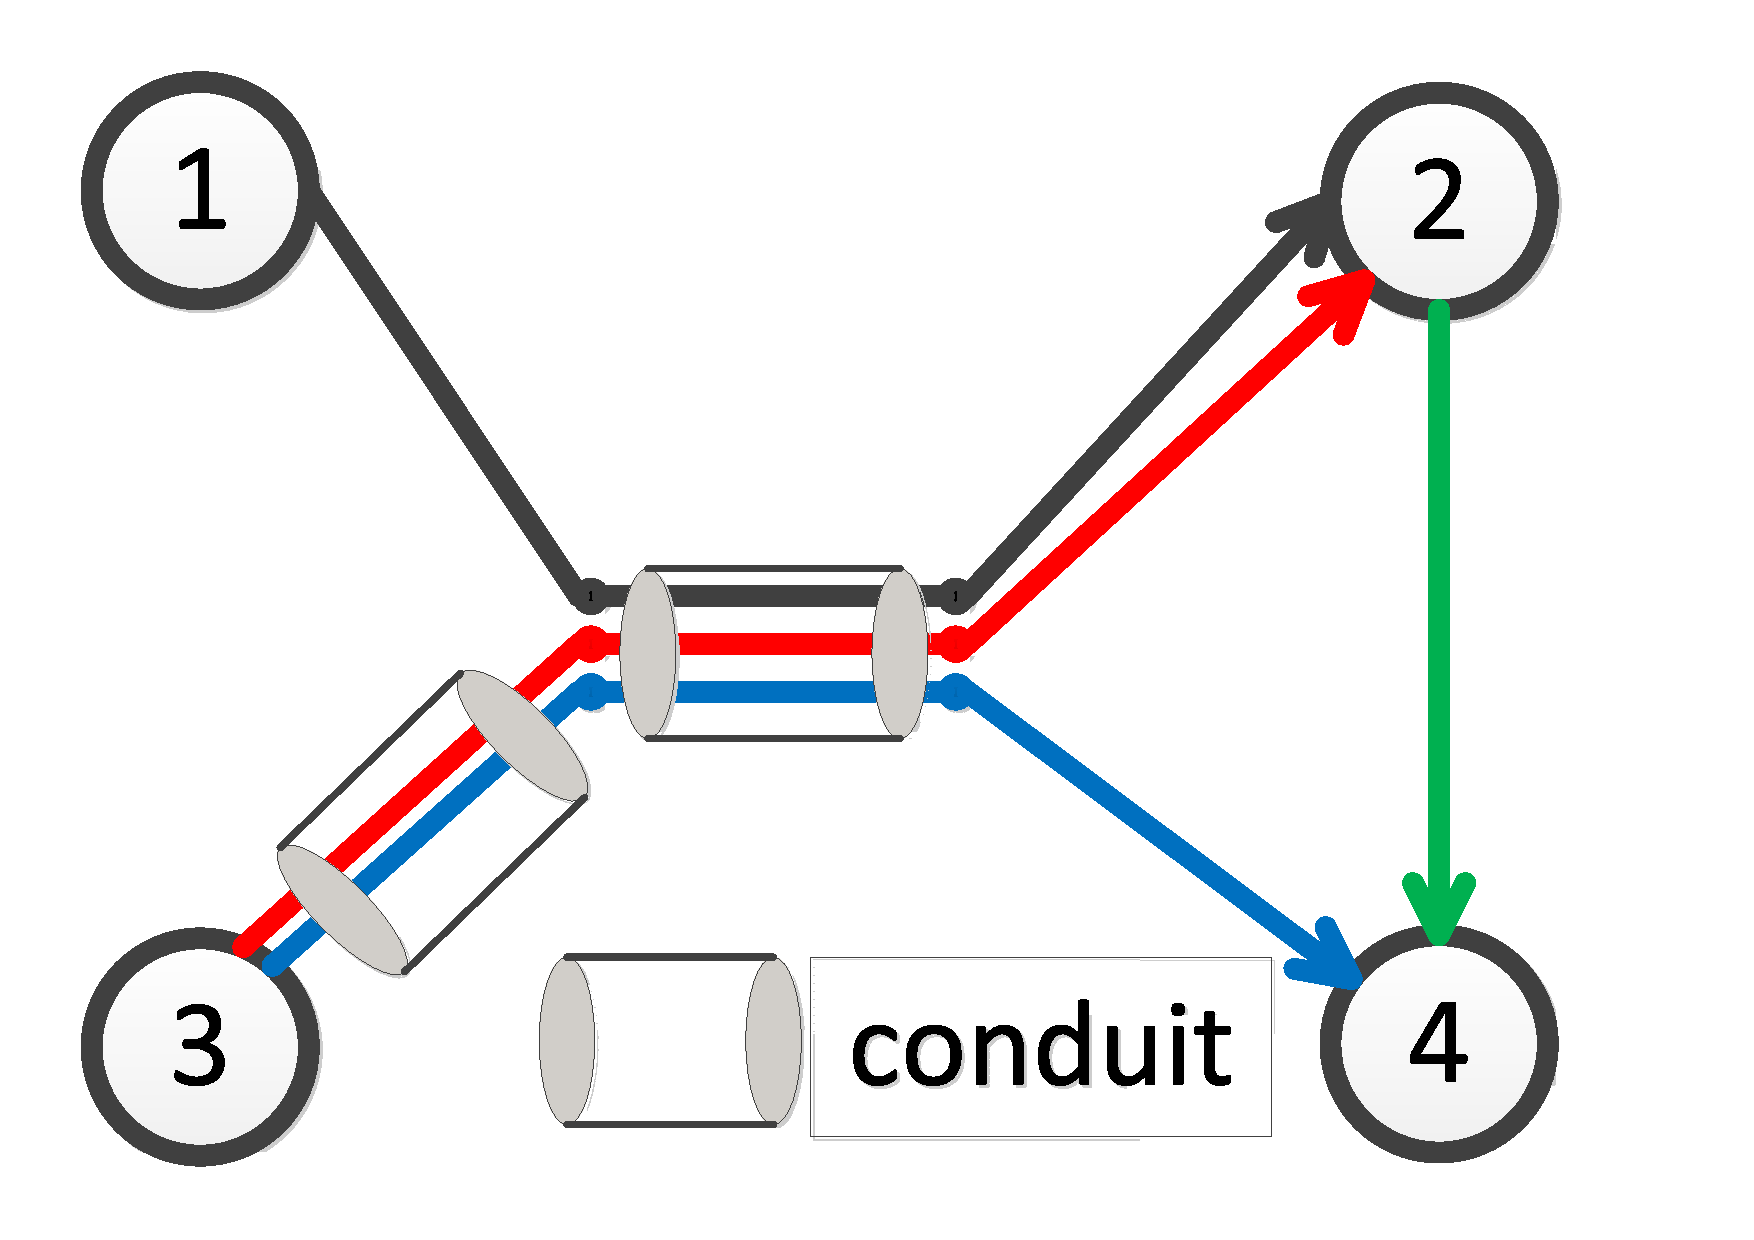
\includegraphics[width=1.25 in]{figures/PhysicalGraph}
}
\subfigure[Network Graph]{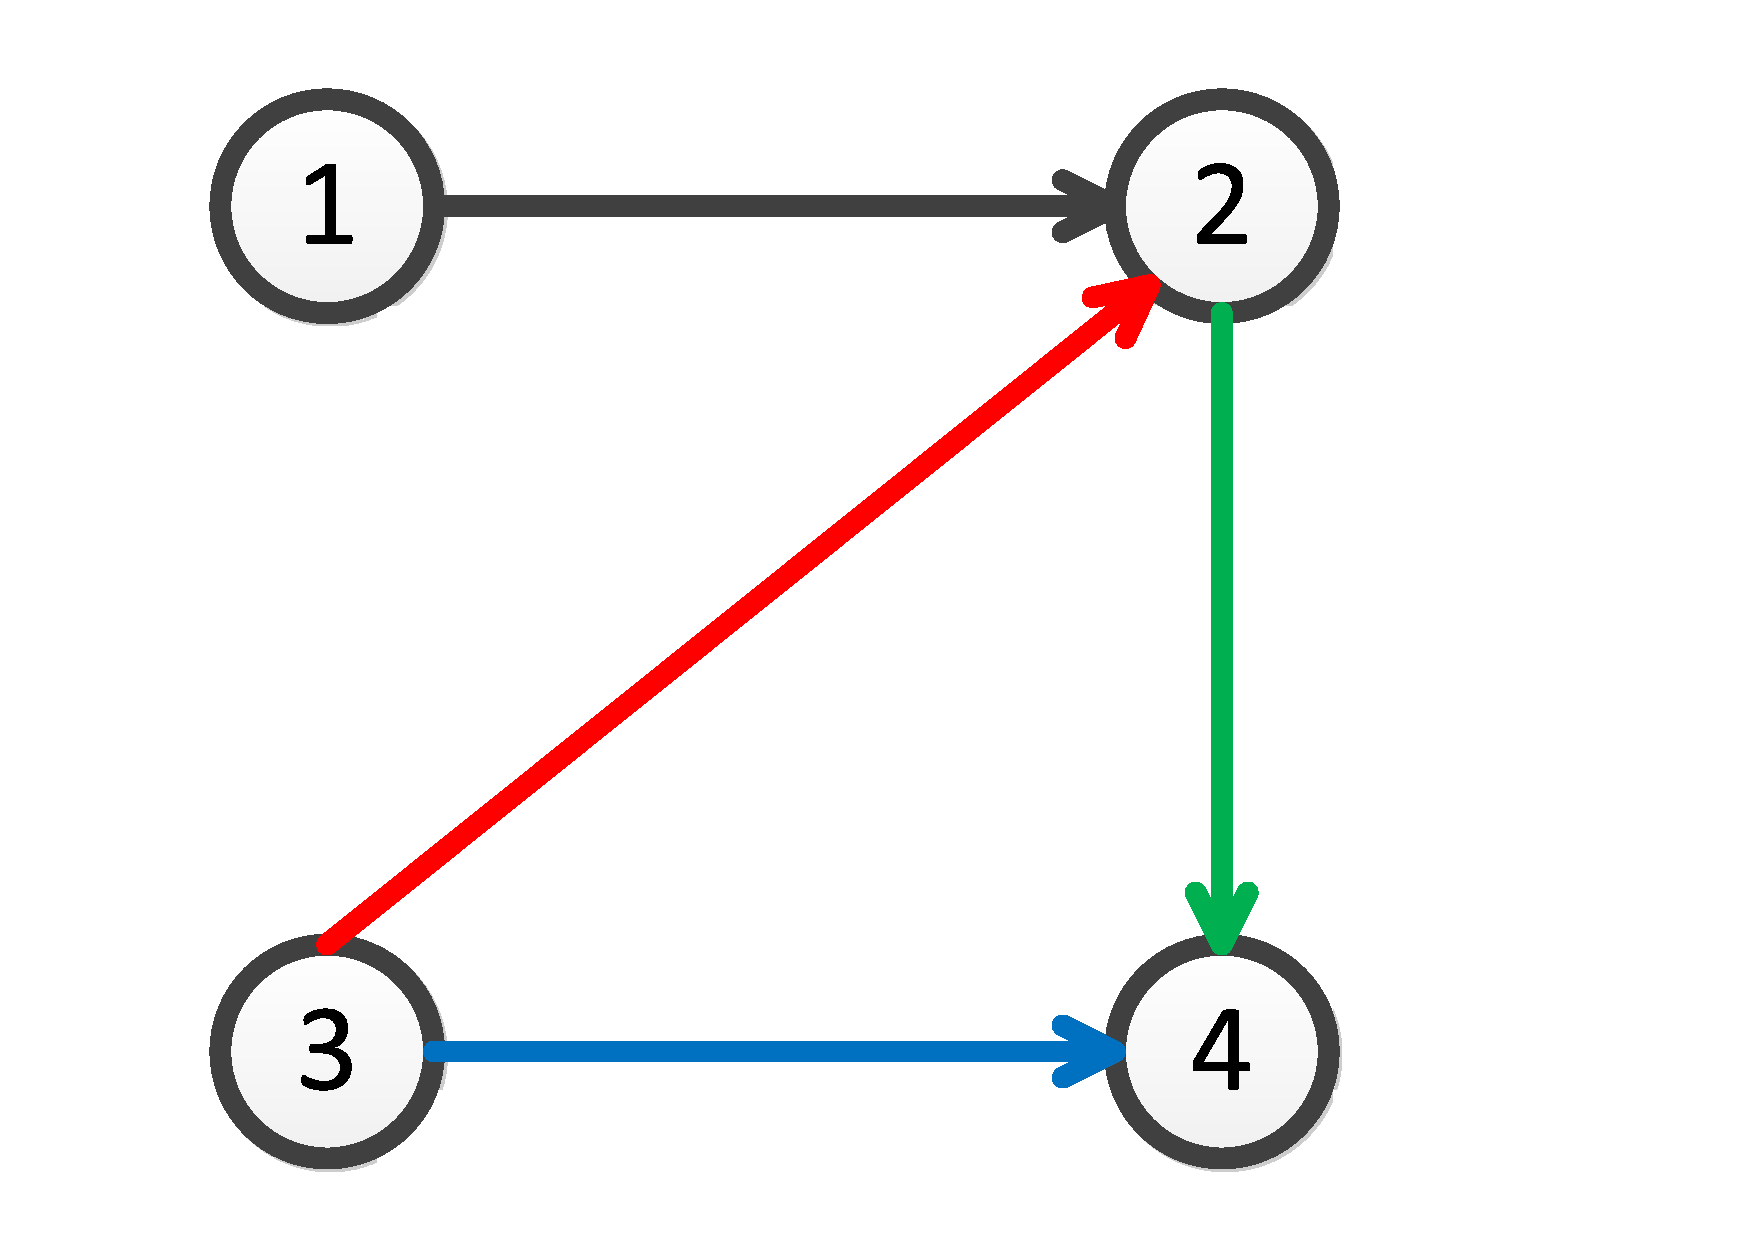
\includegraphics[width=0.9 in]{figures/VirtualGraph}
}
\caption{Example of shared risk link group(SRLG)}\label{fig:SRLGgraph}
\label{fig:Logic shift operation}
\end{figure}

设$\mathbb{R}$为网络中的风险集(故障)。每个风险可能对应于导管断开、光纤断裂、在一个节点上驱动故障、软件故障或这些因素的任何组合。对每一个共享风险链路组$r_i \in \mathbb{R}$ 是指与其风险$r_i$ 相关的链路集合$\mathbb{R}_{r_i}$,$1\leq i\leq \chi$ 和 $\chi=|{\mathbb{R}}|$是共享风险链路组集合的个数。图.\ref{fig:CompositeGraph}(a) 所示,该图包含五个共享风险链路组集合$\mathbb{R}_{r_1}=\{e_1,e_9\}$, $\mathbb{R}_{r_2}=\{e_2,e_3,e_{19}\}$, $\mathbb{R}_{r_3}=\{e_2,e_4,e_{11},e_{17}\}$, $\mathbb{R}_{r_4}=\{e_5,e_{13}\}$, $\mathbb{R}_{r_5}=\{e_{15},e_{18}\}$。 在这个例子中,链路$e_2$同属两个共享风险链路组集合里$\mathbb{R}_{r_2}$ 和 $\mathbb{R}_{r_3}$


$r_P$表示影响路径$P$上的风险集合,即$r_P=\{r\in \mathbb{R}$: 路径 $P$ 包含的链路在 $\mathbb{R}_r$ 中$\}$。 如图.\ref{fig:CompositeGraph}(c) 所示,在路径$AP$ 上的边集$\mathbb{AP}=\{e_1,e_2,e_3,e_4,e_5,e_6,e_7,e_8\}$,并且$e_1\in \mathbb{R}_{r_1}$, $e_2\in \mathbb{R}_{r_2}$, $e_2\in \mathbb{R}_{r_3}$, $e_3\in \mathbb{R}_{r_2}$, $e_4\in \mathbb{R}_{r_3}$, $e_5\in \mathbb{R}_{r_4}$,路径$AP$ 的风险集合是${r}_{{AP}}=\{r_1, r_2, r_3, r_4\}$。$\mathbb{\mathbb{ER}}$ 代表不属于$AP$上的链路但是与$AP$共享相同的风险集合的链路。如图.\ref{fig:CompositeGraph}(c) 所示,$\mathbb{\mathbb{ER}}=\{e_9,e_{11},e_{17},e_{13},e_{19}\}$。


共享风险链路组不相交路径问题定义如下:

\begin{definition}[共享风险链路组不相交路径问题]
给定$|\mathbb{V}|$个节点集$\mathbb{V}$和 $|\mathbb{E}|$条加权链集 $\mathbb{E}$ 组成的有向网络 $G(\mathbb{V},\mathbb{E})$和$|\mathbb{R}|$ 个风险组$\mathbb{R}$,两个特殊节点$s,d\in\mathbb{V}$。 任何链路$(u,v)\in\mathbb{E}$。 给定一个整数$k>0$,求$s$ 到$d$ 的$k$ 条路径$P_1,P_2,\ldots,P_k$,使路径间不共享任何公共风险组。
\end{definition}

共享风险节点组不相交路径可以通过节点转移方法成共享风险链路组不相交路径问题。

%\section{共享风险节点组不相交路径}
\section{本章小结}
表\ref{tab:disjointPath}概述了所考虑的不相交路径问题的变体。每个问题都根据其目的、应用实例和复杂性进行分类。

\begin{table}[htbp]
\caption{不相交路径}\label{tab:disjointPath}
\vspace{0.5em}\centering\wuhao
\begin{tabularx}{46em}{|*{4}{>{\centering\arraybackslash}X|}}
\toprule[1.5pt]
问题   & 限制条件   & 实际应用 & 时间复杂度  \\
\midrule[1pt]
不相交路径 & 路径不共享公用链路p或节点 & 为运输网络中的卡车司机提供不同的候选路径 & 多项式可解(例如Bhandari算法\cite{bhandari1997optimal})\\
\hline
可用性不相交路径 & 路径不共享公共链接或节点,具有可用性约束 & 提高电信网络中业务的连接可用性 & 多项式可解(例如Bhandari算法\cite{bhandari1997optimal})\\
\hline
最大不相交路径 & 路径共享最小的公共链接或节点 & 在两个地点安全地转移一个非常重要的人 & NP难和很难近似到一个因子$2^{log^{1-\epsilon}N}(\epsilon>0)$。当k=2 时,这个问题是多项式可解(例如MADSWIP算法\cite{taft1999quality})\\
\hline
域不相交路径 & 路径不共享公共域 & 提高跨多个光网络域的业务传输可靠性。 & NP难\cite{gao2013domain}\\
\hline
地区不相交路径 & 路径不能受到直径D的单一地区失效的影响(除了包括源或目标节点失效)。 & 确保地区灾难不会同时影响不同不相交的道路 & NP难和很难近似\cite{trajanovski2015finding},除非所有成对的网络节点距离大于$D$。\\
\hline
不相交路径对 & 路径不共享公共链接或节点(路径间可能有不同的源节点和目标节点)。 & 在芯片上互连指定的通道,没有任何不同引脚的电线相互接触 & 当$k\geq2$在一般有向网络中为NP难\cite{fortune1980directed},但在无向网络\cite{robertson1995graph}、有向平面网络\cite{schrijver1994finding}和有向无圈网络中\cite{fortune1980directed}是多项式可解的。 \\
\hline
风险共享链路组不相交路径 & 路径不共享共同的风险组 & 确保不同的不相交路径不使用属于光网络中同一管道的链路。 & NP难\cite{hu2003diverse}和难以近似\cite{coudert2007shared},除非SRLGS 遵循星型性质且SRLGS的数目为常数\cite{bermond2013srlg},或当SRLGS遵循星性且最大节点度最多为4\cite{bermond2013srlg}时,或者当SRLGS 遵循星型性质且网络是有向无圈图\cite{bermond2013srlg}时,或在特定跨度共享拓扑\cite{bhandari1994optimal}中。\\
\bottomrule[1.5pt]
\end{tabularx}
\vspace{\baselineskip}
\end{table}
